\documentclass[12pt]{article}
\usepackage[T1]{fontenc}
\usepackage[utf8]{inputenc}
\usepackage{authblk}
\usepackage{amsfonts}
\usepackage{amsmath,amssymb}
\usepackage{graphicx,xcolor}
\usepackage{hyperref}
\usepackage[export]{adjustbox}
\definecolor{refcol}{rgb}{0.9,0.1,0.1}
\hypersetup{colorlinks=true,linkcolor=blue,citecolor=refcol,urlcolor=cyan,linktocpage}
\begin{document}
\begin{titlepage}
    \title{
        {\huge\bf\color{blue}On a new field theory formulation and a space-time adjustment that
        predict the same precession of Mercury and the same bending of light
        as general relativity}\\
        \author{{\bf Sayan Sarkar} \footnote{{\tt\color{red} williamskyle562@gmail.com}}\hspace{8pt} 
        \hfill\\
        \centering
        {\large\bf{Department of physics}}\\ \bigskip
        {\Large\bf{Ashutosh College}}\\ \bigskip
        {\it\large 92 Shyama Prasad Mukherjee Road,Jatin Das Park,Patuapara,Bhowanipur}\\
        {\it\small Kolkata 700026, India} \bigskip
        \hfill\\        
        \centering      
        {\it\large affiliated to :- \\ Calcutta University }
        \hfill\\
        \centering
        \begin{figure}[htbp]
            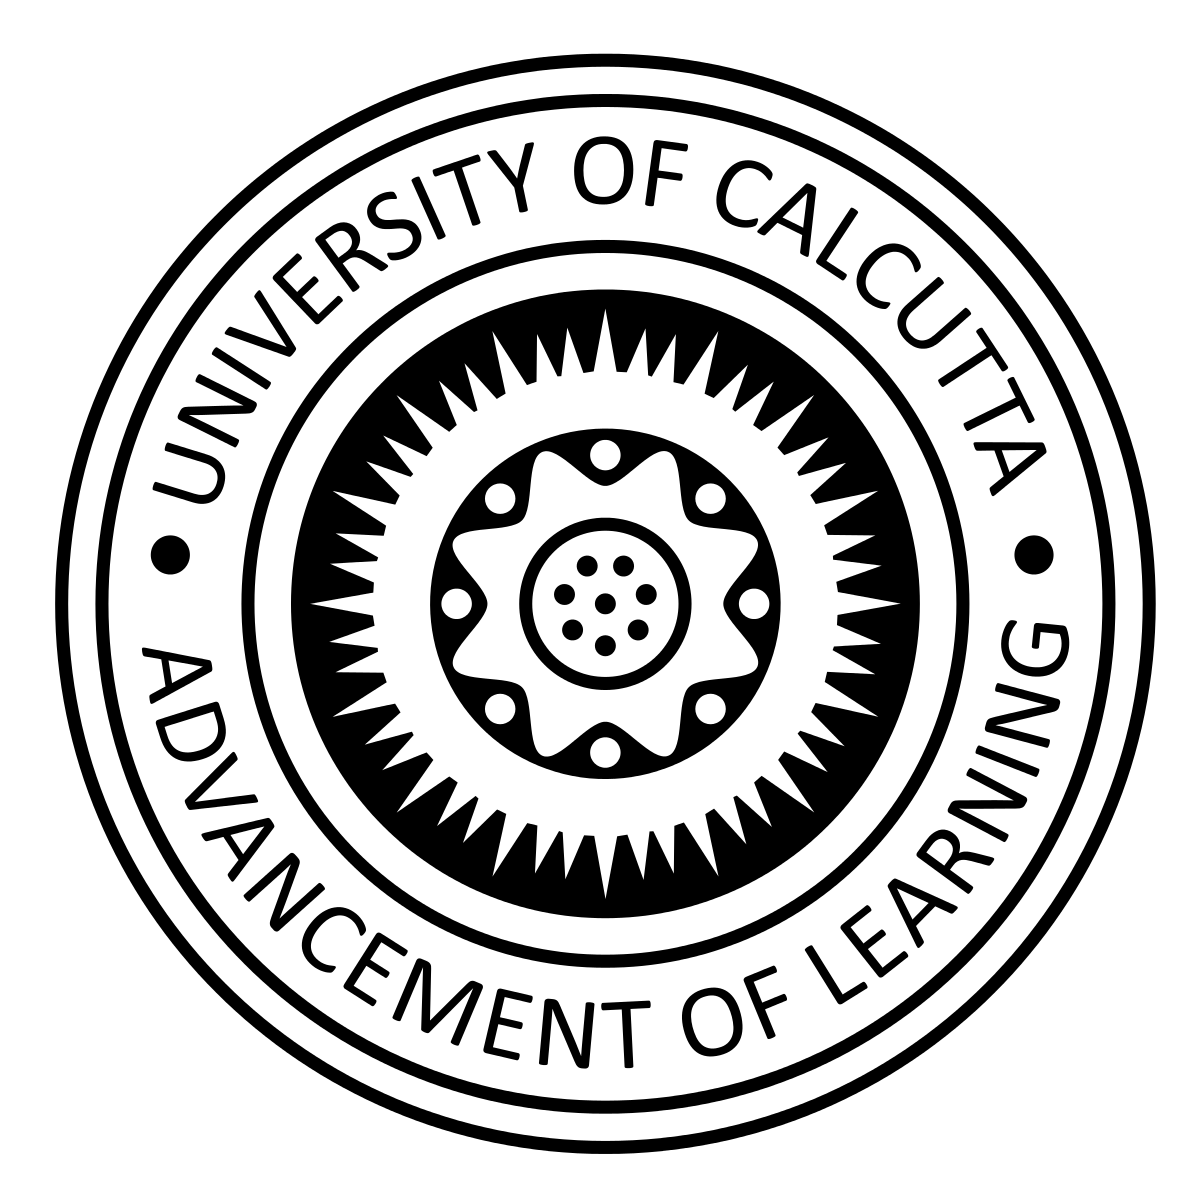
\includegraphics[width=0.4\linewidth, center]{calc.png}
        \end{figure}
        \newpage
        \textbf{Abstract:}
         This article introduces a new field theory formulation. The new field theory formulation
        recognizes vector continuity as a general principle and begins with a field that satisfies vector
        continuity equations. Next, independent of the new formulation, this article introduces a
        new space-time adjustment. Then, we solve the one-body gravitational problem by applying the
        space-time adjustment to the new field theory formulation. With the space-time adjustment,
        the new formulation predicts precisely the same precession of Mercury and the same bending
        of light as general relativity. The reader will find the validating calculations to be simple.
        The equations of motion that govern the orbital equations are in terms of Cartesian coordinates
        and time. An undergraduate college student, with direction, can perform the validations.
         2020 Physics Essays Publication. 
        [\url{[http://dx.doi.org/10.4006/0836-1398-33.4.489]}
        }     
        }
\end{titlepage}
\maketitle\vfill \eject
\tableofcontents
\section{Introduction}\label{sec:Intro}
One describes mathematically any space-time field that
has flow lines that never begin, nor end, nor cross, as a fourdimensional vector function that satisfies vector continuity
equations. The vector continuity equations are general equations that reduce to conservation laws,
to wave equations, and to potential equations. Therefore, in
retrospect, it was never a coincidence in Newtonian theory
(NT) that the gravitational potential satisfies potential equations. It was never a coincidence in electromagnetic theory
(EM) that Maxwell’s equations describe fields that satisfy
wave equations within a given frame of reference. Vector
continuity appears throughout NT, EM, and special relativity
(SR). One of the novelties of the new FT formulation is that
it begins with vector continuity.
NT, EM, SR, and general relativity (GR) claim different
territories in the landscape of physics, and their territories overlap. The formulations differ by their metrics, by their
frames of reference, and by their coordinate systems. Scientists have attempted to connect one theory to the other. For
example, as it pertains to the connection between NT and
GR, Atkinson1 examined GR in Euclidean terms and Montanus2 developed a formulation of GR in so-called absolute
Euclidean space-time. Sideris asked fundamental questions
about the connections between NT and GR, and Ziefle4 modified NT by the introduction of “gravitons” in an attempt to
predict the precession of Mercury and the bending of light.
These and other researchers strengthened the belief that
important connections exist between NT, EM, SR, and GR.
\begin{figure}[htbp]
    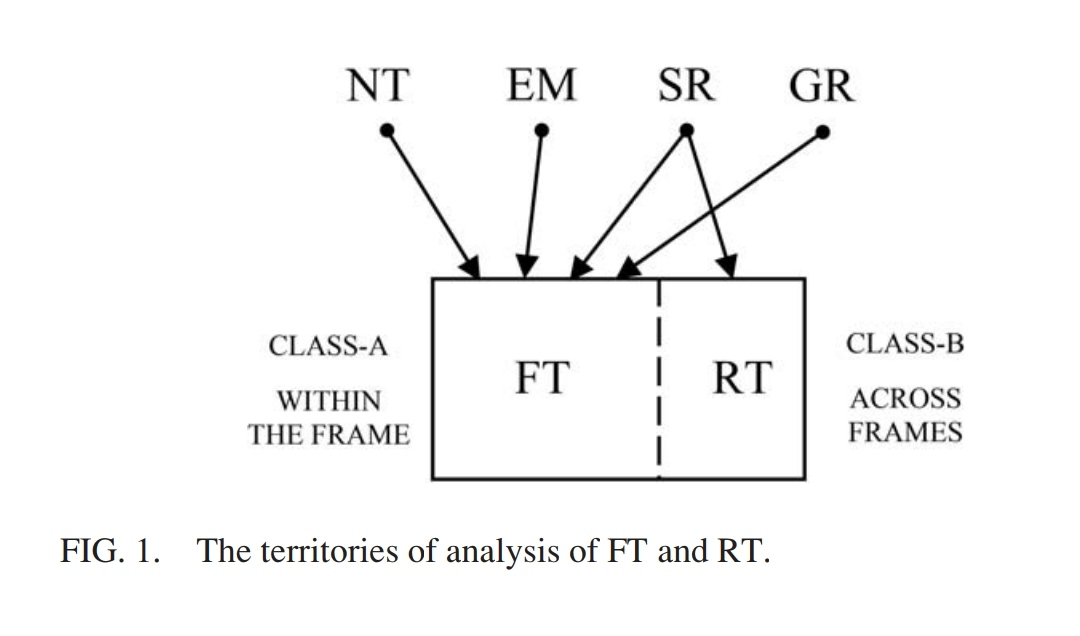
\includegraphics[width=0.6\linewidth]{1.jpg}
\end{figure}
However, the connections continue to be confusing, and the
work is not complete.To address this confusion, let us now distinguish
between two classes of physical theories: The class-A theory
addresses physical behavior within a frame of reference, and
the class-B theory addresses physical behavior across two or
more frames of reference. This article focuses on the class-A
theory, in particular, the new FT formulation and on a new
space-time adjustment that we apply to gravitation in the 
new FT formulation. We will refer to the class-B theory as
relativity theory (RT). To be clear, by frame of reference, we
mean the frame in which one takes measurements and makes
observations. This is quite different from what one means by
the coordinate system. One can employ different coordinate
systems within a frame of reference, and one can employ the
same coordinate system across different frames of reference
at the instant the frames are coincident. One employs the
Galilean transformation between coordinate systems within a
frame of reference and the Lorentz transformation across
frames of reference regardless of the coordinate system .

\section{Introduction to new FT formulation}
Before proceeding to the validations, we briefly introduce the new FT formulation and compare it with the
present-day formulation. The present day formulation starts
with a relativistic correction in inertial space of the law of
inertia in NT; the present-day field theory is a relativistic
NT. It replaces the law 
$F \textsubscript{r} = m\frac{dv}{dt} v \textsubscript{r} $ (r = 1,2,3,4...)
 which
describes the interaction force vector responsible for changing the state of a particle, with the relativistic law

$F \textsubscript{r} = m\frac{dv}{dt} (\frac{v \textsubscript{r}}{\sqrt{1-(\frac{v}{c})^2} } ) (r=1,2,3,4,...)$ \\
Notice in the law
of inertia, with and without the relativistic correction,
that one obtains the force vector by time differentiation.
Furthermore, notice that the relativistic velocity components
$(\frac{v \textsubscript{r}}{\sqrt{1-(\frac{v}{c})^2} } ) (r=1,2,3)$
align with the first three
components of a 4D unit vector that is tangent to the particle’s space-time path. The authors characterize the presentday field theory as intending to accommodate the transition
from the particle to the field and from the spatial domain to
the space-time domain. We now contrast the present-day formulation with the new formulation.
\section{Three Formulation}
The fundamental problem of gravitation is a two-body
problem. Whether employing FT, NT, or GR, one
converts the two-body problem into a one-body problem
(Appendix B). The following compares the treatments of the
one-body problem in FT and NT with its treatment in GR.
As will be seen below, the treatments require a space-time
adjustment. Table I lists the fragment of energy, energy,
action force, and interaction force for the one-body gravitational problem and more generally the governing equations
(change equations and laws of inertia). For the one-body
gravitational problem, the orbital mechanics takes place in
the x\textsubscript{1},x\textsubscript{2} plane, the mass of the sun is M, and the mass of the
orbiting body is m, where the orbiting body is either Mercury
or a photon.
\subsection{Gravitation in the new FT formulation with no
space-time adjustment}
In the one-body gravitational problem, the field consists
of just one fragment of energy. TABLE Ia gives its components. The term A given there is the magnitude of the vector
field with components A\textsubscript{s} (s=1,2,3,4) Next, an action
force is determined. Then, one determines 4D curvature vector components k\textsubscript{s}(s=1,2,3,4)
by substituting the action
force vector into the change equation.
\subsection{Gravitation in the new FT formulation with a
 space-time adjustment}
 Table Ib gives the components A\textsubscript{s} (s=1,2,3,4) of the
vector field of a stationary fragment using a space-time
adjustment that we introduce for gravitation. We first apply
it here to the new FT formulation and later to NT. The
space-time adjustment adjusts the relationship between the
speed of the source point of the orbiting fragment upon
which the field of a stationary fragment acts, such as
Mercury or a photon, and the orbiting fragment’s corresponding angular momentum. Start by considering the circular motion of an orbiting fragment. In FT, the following
expression is exact for circular motion:
\\
$\frac{1}{1-(\frac{v}{c})^2}=1+(\frac{h}{mc})^2\frac{1}{r^2} (where,  h=\frac{mrv}{\sqrt{1-(\frac{v}{c})^2} })$
 \subsection{Gravitation in  NT with no space-time adjustment }
 NT with no space-time adjustment
begins with a potential energy function V or with interaction
force vector components F\textsubscript{s} (s=1,2,3)  A gradient vector
relates the two by $ F\textsubscript{s}=-\frac{\partial v}{\partial x\textsubscript{s}} (s=1,2,3)$
Then, one
determines 3D acceleration vector components a\textsubscript{s} (s=1,2,3)
) by substituting the interaction force vector into the governing law of inertia. Note that the potential energy function
in NT with no space-time adjustment is not associated with a
potential energy vector function. The potential energy function for gravitation will recognize that V is associated with a
potential energy vector function.
 \subsection{Gravitation in NT with space-time adjustment}
 We begin with NT and now associate the potential energy
V of a body with a potential energy vector function like in the
new FT formulation. Next, we apply the space-time adjustment to the one-body gravitational problem in NT. Again, the
space-time adjustment considers the relationship between the
speed of the mass center of the orbiting body and its corresponding angular momentum and, again, we start by considering the circular motion of the orbiting body. In NT, the
following expression is exact for circular motion: \\
$\frac{1}{1-(\frac{v}{c})^2}=1+(\frac{H}{mc})^2\frac{1}{r^2} (where,H=rmv)$
where H is the angular momentum of the orbiting body. The
space-time adjustment consists of first multiplying the gravitational potential $-GM\frac{1}{r}$ of the stationary body
Again, in the one-body gravitational problem, the
speed v of the orbiting body is not constant whereas its angular momentum is constant. Again, when one multiplies the
gravitational potential $-GM\frac{1}{r} $by the right side of the first
expression in above equation, one finds that the expression splits into
two parts, with H being constant . Like in
FT, the second step is to replace the left side of above equation with the right side of Eq.
which eliminates the dependence on
v and expresses V in terms of its independent spatial coordinates alone. We determine the interaction force by the sun
from $F\textsubscript{r} =-\frac{\partial v}{\partial x\textsubscript{r}}(r=1,2,3)$ ; holding H constant.
Again, we used the resulting expression to determine the
interaction force at any point along the trajectory wherein
the motion is not circular .Again, we no longer guarantee vector continuity to be satisfied after making the adjustment.
In this article, the reader will discover, had Newton
added the previously mentioned second term in last eq. to the
gravitational potential, that he would have predicted the
same precession of Mercury as in GR. On the other hand, he
would not have been inclined to pursue that because during
the time of Newton scientists had not yet observed the precession of Mercury, they had not yet developed the concept
of vector continuity, nor had scientists yet developed the
apparatus of curved space-times .
\section{Results}
A body orbits the sun in the problem of the precession of
Mercury and in the problem of the bending of light. In the
bending of light problem, the body is a massless point traveling at the speed of light. One calls such a point a photon .
each problem, we determined the trajectories by numerical
integration of the accelerations of the orbiting body. We
adopted a numerical approach instead of an analytical
approach, because analytical results do not yet exist for all of
the cases considered and because the numerical approach
simplifies the verification of the results. 
\begin{table}[h!]
    \centering
    \caption{Physical Constants}
    \begin{tabular}{ccc}
    \hline
         \multicolumn{3}{c}{sun}  \\
         \hline
         M & Mass of the sun & $1.989\times10\textsuperscript{39}$ Kg \\
         \hline
         r\textsubscript{s} & Radius of Sun & 696 000 000m \\
         \hline
    \end{tabular}
    \label{tab:my_label}
\end{table}

\begin{table}[h!]
    \centering
    \begin{tabular}{ccc}
         \multicolumn{3}{c}{Mercury}  \\
         \hline
         m & Mass of the Mercury & $3.3\times10\textsuperscript{23}$Kg \\
         \hline
         r\textsubscript{p} & periphelion radius of Mercury & $4.6\times10\textsuperscript{10}$m \\
         \hline
         r\textsubscript{b} & Aphelion radius of Mercury & $6.982\times10\textsuperscript{10}$m \\
         \hline
         A & Semimajor axis of Mercury & $57.91\times10\textsuperscript{9}$m \\
         \hline
         e & Eccentricity of Mercury & 0.20566\\
         \hline
         v\textsubscript{p} & Perihilion Velocity & $58.98\times10\textsuperscript{3}$m/s\\
         \hline
         T & Orbital Period & $ 87.969 Earth Days=7600530 $s \\
         \hline
    \end{tabular}
    \label{tab:my_label}
\end{table}

\begin{table}[h!]
    \centering
    \begin{tabular}{ccc}
         \multicolumn{3}{c}{Other}  \\
         \hline
         G & Gravitational Constant & $6.674\times10\textsuperscript{-11}$$\frac{m\textsuperscript{3}}{kg-s^2}$\\
         \hline
         c & Speed of Light & $2.99\times10\textsuperscript{8}$m/s\\
         \hline 
    \end{tabular}
    \label{tab:my_label}
\end{table}


 \subsection{Precision of Mercury}
 GR predicted successfully the so-called anomalous precession of Mercury, over and above the precession caused by
the other planets and solar oblateness. From GR, the analytically determined precession of Mercury is \\
$\delta \varphi  =\frac{6\pi G(M+m)}{c^2 A(1-e^2)} \\
=5.07\times 10\textsuperscript{-7}   rad/orbit \\
=0.104093  arc-sec/orbit \\
=43.2  arc-sec/century \\
$
Again, the numerically integrated trajectories began at
Mercury’s perihelion with the initial conditions.
\begin{figure}[htbp]
    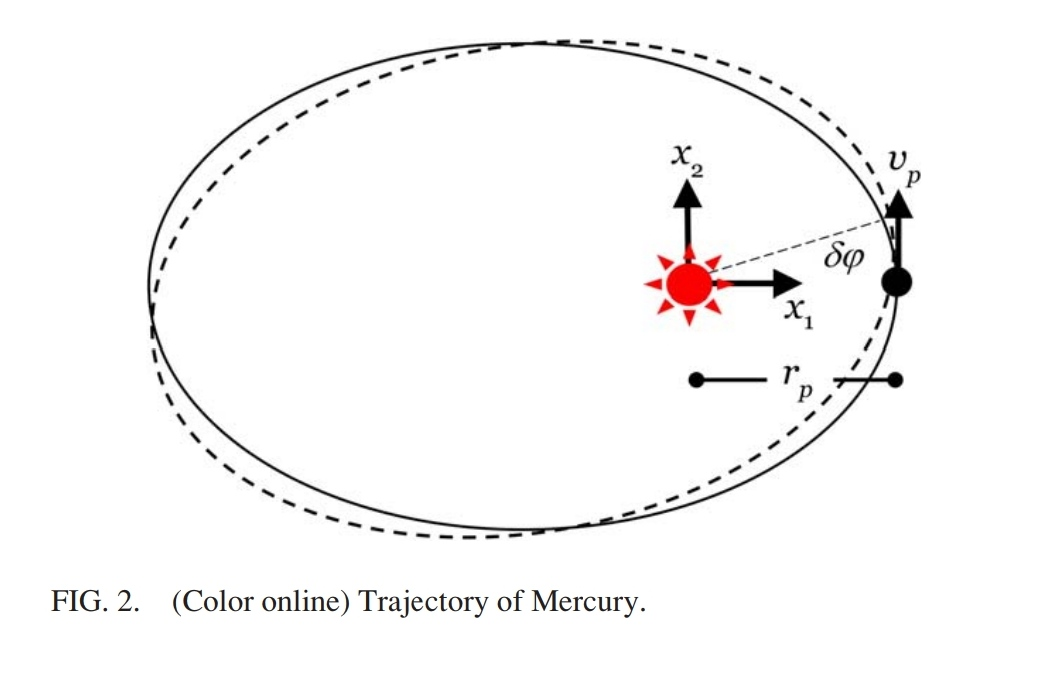
\includegraphics[width=0.6\textwidth, right]{IMG_20210218_183609.jpg}
\end{figure}
In order
to determine the precise location of the next perihelion, the
time derivative of the orbit radius 
$\frac{dr}{dt}=\frac{(x\textsubscript{1}\frac{dx\textsubscript{1}}{dt}+x\textsubscript{2}\frac{dx\textsubscript{2}}{dt})}{r} $
was monitored, and the time when its value crossed zero was
determined. At that instant, the predicted angle of precession
was calculated numerically from $\delta \varphi = \frac{x\textsubscript{2}}{r\textsubscript{p}}$ \\


\subsection{Bending of light}
 The classic problem of analytically determining the
bending of light by GR predicts the angle of bending as 
$\delta\textsubscript{N}=\frac{4GM}{c^2 r\textsubscript{p}} \\
=8.534\times 10\textsuperscript{-6} rad \\
= 1.706arc-sec$

where r\textsubscript{p} is the “distance of closest approach” (the perihelion) and, for the purposes of simulation, has been set equal
to the radius r\textsubscript{s} of the sun . In order to predict the
path of a photon orbiting the sun, we considered the model
of a photon using the equations of motion . First,
we set $ \mu =\frac{mM}{m+M}$ Þ to m after which the m cancelled
from the equations of motion. In FT with the adjustment, by
setting the photon speed to the speed of light, one would get
a divide by zero error .
\begin{figure}[htbp]
    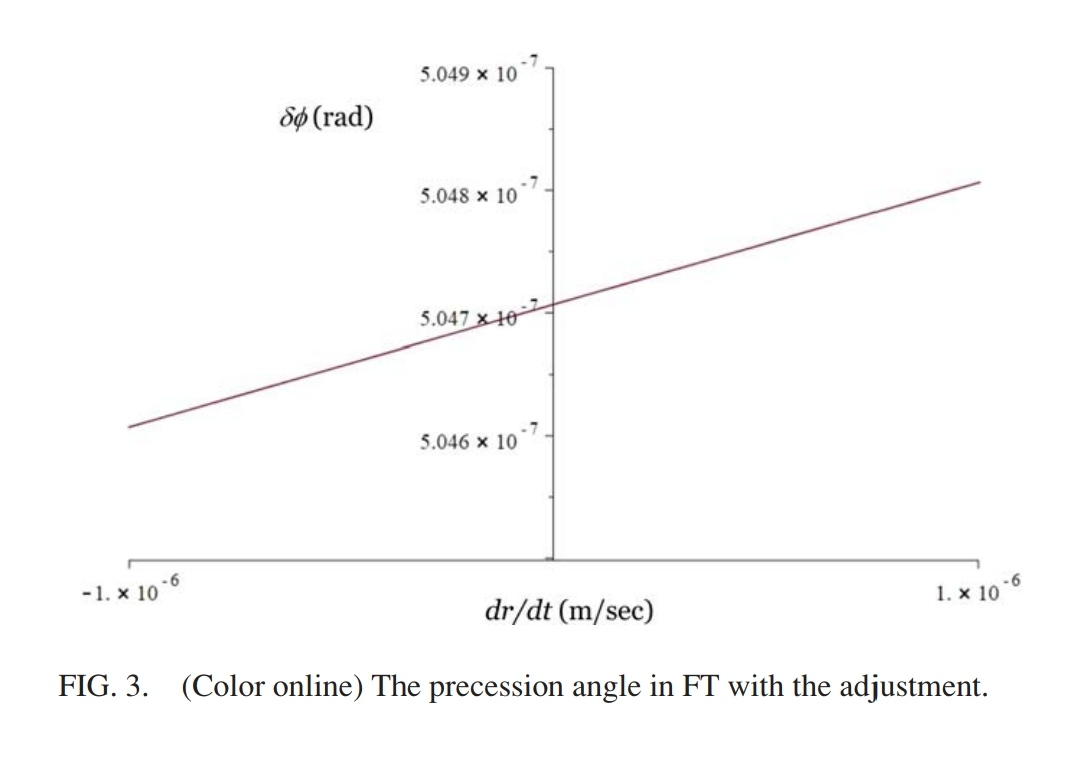
\includegraphics[width=0.6\linewidth]{IMG_20210218_183628.jpg}
\end{figure}
The divide by zero arises in the
term $(\frac{h}{mc})^2 = (\frac{r\textsubscript{s}v\textsubscript{2}}{c})^2 \frac{1}{1-(\frac{v}{c})^2}$
when v is set equal to c.
The expressions for the acceleration components become
indeterminate ), so we take the limit as v approaches c
instead of evaluating v at c. The bending angle of light numerically
determined by FT with the adjustment for increasing initial
photon speeds. For an initial speed equal greater than or
equal to 0.9999c, the predicted numerical value agrees to
three decimal places with the celebrated analytical result.
\begin{figure}[htbp]
    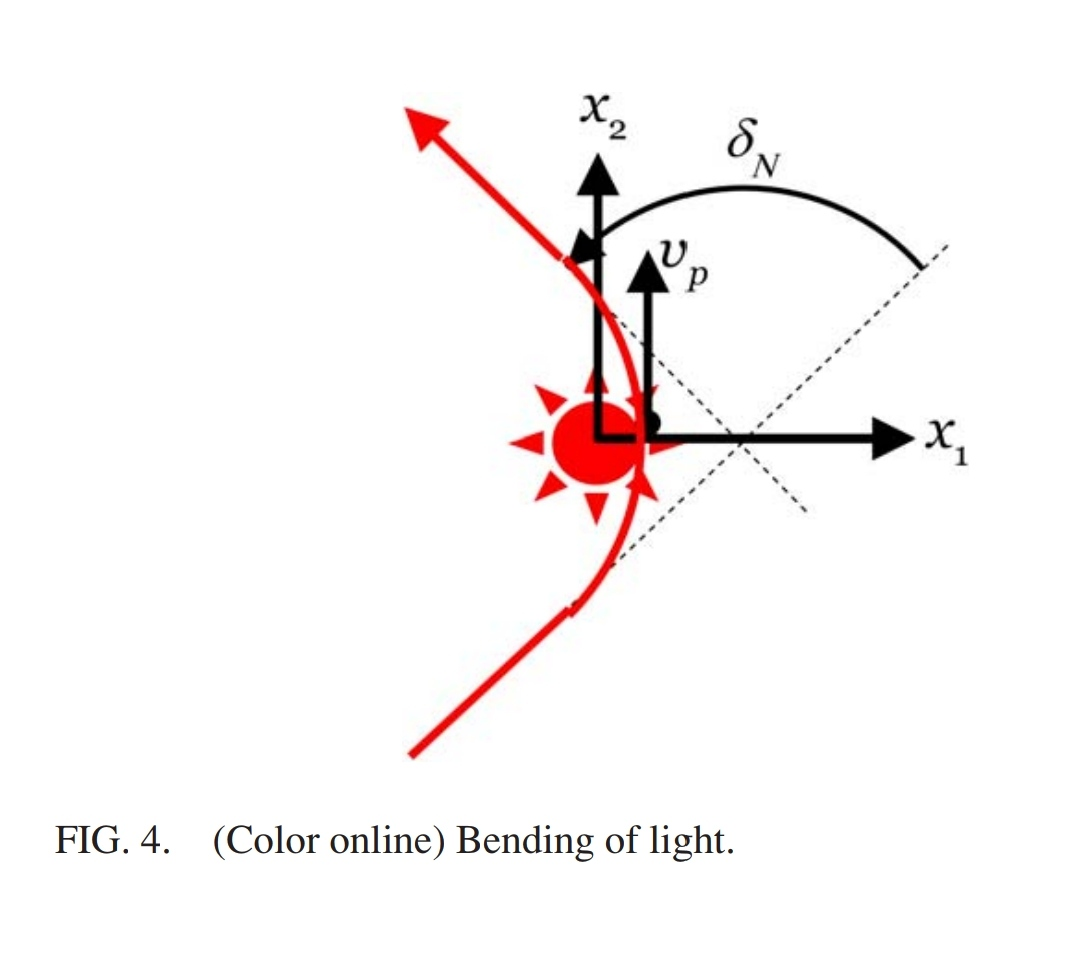
\includegraphics[width=0.6\linewidth, right]{IMG_20210218_183644.jpg}
\end{figure}
FT without the adjustment predicts
a bend angle of precisely zero.
\begin{figure}[htbp]
    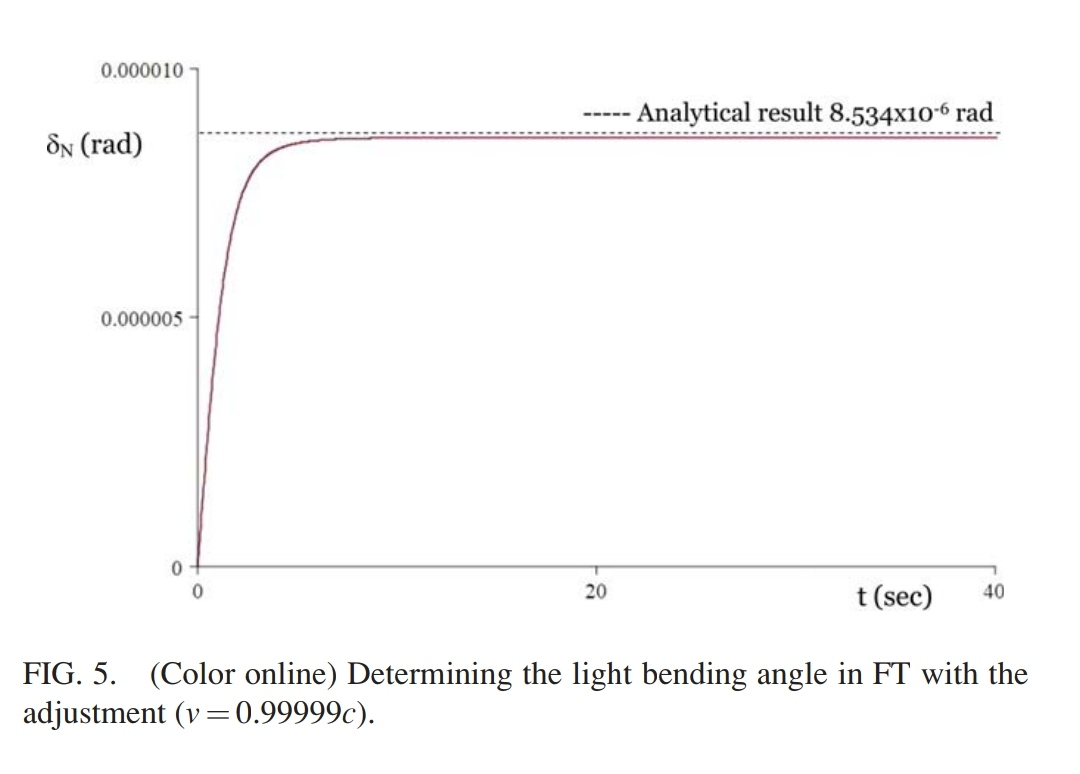
\includegraphics[width=0.6\linewidth]{IMG_20210218_183705.jpg}
\end{figure}
In contrast, NT without the
adjustment predicts a bend angle that is precisely 50\%
smaller than the bend angle that GR predicts. This result is
well-known.
Notably, with the space-time adjustment, FT
predicts precisely the same bending of light that GR predicts
in addition to precisely the same precession of Mercury that
GR predicts ,respectively, predicts precisely 50\% less and then precisely
50\% more bending of light than GR predicts. \\

\section{Summary}
Think of energy as made up of lines that fill up a region of space and time,
flowing into and out of that region, never beginning,
never ending and never crossing one another.
Even though, mathematically, there were lots of robust contenders,
We can chose a concentration (or fragments) of energy as the building block.
Such fragments have the properties of both particles and waves, with the highest concentration of energy at the centre,
which dissipates as it moves further away.

While standard physics work perfectly fine in most cases,
things often become much trickier when it comes to the very large and the very small scale.

Modelling the celestial bodies as fragments of energy, we can finf
that the are identical to those predicted by the theory of general relativity.

\section{Conslusion}
The fragment could be a single potentially universal building block from which to model
reality mathematically – and update the way people think about the building blocks of the Universe.
\newpage
\begin{thebibliography}{9}
    \bibitem{latexcompanion} 
    Larry M. Silverberg and Jeffrey W. Eischen
    \textit{The \LaTeX\ Companion}. 
    Department of Mechanical and Aerospace Engineering, North Carolina State University,
    Campus Box 7910,
    Raleigh, North Carolina 27695-7910, USA
    \bibitem{latexcompanion} 
    Wikipedia, Sun, [Online]. Available: [\url{https://en.wikipedia.org/wiki/Sun}]
    \bibitem{latexcompanion} 
    Wikipedia, Mercury (planet), [Online]. Available: [\url{https://en.wikipedia.org/wiki/Mercury_(planet)}]
    \bibitem{latexcompanion} 
    David R. Williams, NASA Goddard Space Flight Center,[\url:{https://nssdc.gsfc.nasa.gov/planetary/factsheet/mercuryfact.html}]
    \bibitem{latexcompanion} 
    Wikipedia, Gravitational constant, [Online]. Available:[\url{https://en.wikipedia.org/wiki/Gravitational_constant}]
    \bibitem{latexcompanion} 
    Wikipedia, Speed of light, [Online]. Available: [\url{https://en.wikipedia.org/wiki/Speed_of_light}]
    \bibitem{latexcompanion} 
    Wikipedia, “Two-body problem in general relativity,” [Online]. Available:
    [\url{https://en.wikipedia.org/wiki/Two-body_problem_in_general_relativity}]
    \bibitem{latexcompanion} 
    Wikipedia, “Schwarzschild geodesics,” [Online]. Available: [\url{https://en.wikipedia.org/wiki/Schwarzschild_geodesics}]
    \bibitem{latexcompanion}
    Physics Essays:[\url{http://dx.doi.org/10.4006/0836-1398-33.4.489}]
\end{thebibliography}
\end{document}

